% COP-RFS: IEEE Transactions on Signal Processing, 2026
\documentclass[journal]{IEEEtran}

\usepackage{amsmath,amssymb,amsfonts}
\usepackage{algorithmic}
\usepackage{algorithm}
\usepackage{graphicx}
\usepackage{textcomp}
\usepackage{xcolor}
\usepackage{cite}
\usepackage{bm}
\usepackage{multirow}
\usepackage{booktabs}
\usepackage{subfig}
\usepackage{hyperref}
% \usepackage{placeins} % Removed: FloatBarrier causes excessive whitespace

% Custom commands
\newcommand{\vect}[1]{\boldsymbol{#1}}
\newcommand{\mat}[1]{\mathbf{#1}}
\newcommand{\E}{\mathbb{E}}
\newcommand{\R}{\mathbb{R}}
\newcommand{\C}{\mathbb{C}}
\newcommand{\Tr}{\mathrm{Tr}}
\newcommand{\diag}{\mathrm{diag}}
\newcommand{\Real}{\mathrm{Re}}
\newcommand{\Imag}{\mathrm{Im}}
\DeclareMathOperator*{\argmin}{arg\,min}
\DeclareMathOperator*{\argmax}{arg\,max}

\begin{document}

\title{A Closed-Loop Subspace--RFS Framework for\\DOA Estimation and Multi-Target Tracking}

\author{Jin~Ho~Choi,~\IEEEmembership{Member,~IEEE}
\thanks{J.~H.~Choi is with SmartEAR AI, Daegu, South Korea (e-mail: jinhochoi@smartear.co.kr).}
\thanks{Manuscript received XXXX XX, 2026; revised XXXX XX, 2026.}}

\markboth{IEEE TRANSACTIONS ON SIGNAL PROCESSING, VOL.~XX, NO.~XX, 2026}
{Choi: A Closed-Loop Subspace--RFS Framework for DOA Estimation and Tracking}

\maketitle

\begin{abstract}
We present a closed-loop subspace--RFS framework that couples direction-of-arrival (DOA) estimation with random-finite-set (RFS) multi-target tracking and, unlike prior open-loop cascades, analyzes the coupling itself. The closed loop is \emph{front-end-agnostic}: the tracker's temporal prediction is fed back to refine the signal subspace of any subspace DOA estimator. We instantiate it with a higher-order-cumulant front-end (COP, which extends operation to the underdetermined regime $K>M{-}1$; the resulting tracker is COP-RFS) and a covariance front-end (MUSIC). Our central contributions are theoretical: (i)~a posterior Cram\'{e}r--Rao bound for the \emph{complete closed-loop} estimator--tracker, proving the temporal prior restores identifiability exactly where the data-only bound diverges; and (ii)~a recasting of the subspace refinement as minimum-variance inverse-variance fusion on the Grassmann manifold, with a validation gate guaranteeing the loop never degrades performance. The framework is also \emph{back-end-agnostic}, integrating track-oriented PHD, labeled multi-Bernoulli (LMB), and $\delta$-GLMB filters. Monte-Carlo experiments (up to $500$ trials, $95\%$ confidence intervals) show that COP-RFS detects significantly more targets than a MUSIC--PHD baseline when $K>M{-}1$, and that the gated loop lowers low-SNR localization error by up to $56\%$ for both front-ends while cutting moving-target identity switches by $15\%$, matching the open-loop baseline otherwise. We delineate the operating regime in which the higher-order front-end is advantageous rather than claiming uniform superiority.
\end{abstract}

\begin{IEEEkeywords}
Direction-of-arrival estimation, high-resolution, higher-order cumulants, underdetermined systems, multi-target tracking, probability hypothesis density filter, random finite sets, constrained optimization.
\end{IEEEkeywords}

\section{Introduction}
\label{sec:intro}

High-resolution direction-of-arrival (DOA) estimation is a fundamental problem in array signal processing with critical applications in radar, sonar, communications, and defense systems~\cite{barshalom2011tracking,neri2018defense}. Classical high-resolution subspace methods such as MUSIC~\cite{schmidt1986music}, ESPRIT~\cite{roy1989esprit}, and Capon's MVDR beamformer~\cite{capon1969mvdr} achieve super-resolution beyond the Rayleigh limit but are restricted to the \emph{overdetermined} case where the number of sources $K$ does not exceed $M-1$, the number of sensors minus one. This constraint poses a significant challenge in modern defense scenarios where a sensor array may face more incoming threats than its aperture can nominally resolve.

Higher-order statistics (HOS) offer a principled approach to overcome this limitation~\cite{porat1991doa,chevalier2006hos}. By exploiting the $2\rho$th-order cumulant structure of received signals, Choi and Yoo~\cite{choi2015underdetermined} proposed a high-resolution Subspace Constrained Optimization of the Pseudo-spectrum (COP) algorithm, which extends the effective array aperture through a \emph{virtual array} of size $M_v = \rho(M-1)+1$, thereby resolving up to $\rho(M-1)$ sources---far exceeding the classical $M-1$ limit. Alternative approaches to the underdetermined DOA problem include sparse array designs such as nested arrays~\cite{pal2010nested} and coprime arrays~\cite{vaidyanathan2011coprime,liu2018superresolution,zhou2018deformed}, as well as sparsity-based and sparse-Bayesian-learning methods~\cite{malioutov2005l1svd,wipf2004sbl,gerstoft2016sbl}. However, these approaches either require specialized array geometries or assume signal sparsity, whereas COP operates on standard ULAs and exploits higher-order cumulant structure. A key advantage of higher-order cumulants is the automatic suppression of Gaussian noise, since all cumulants of order greater than two vanish for Gaussian processes~\cite{mendel1991tutorial}---a robustness that holds even for spatially-colored, unknown noise. These strengths come at the cost of higher estimation variance; a central premise of this work is that embedding HOS \emph{within a closed loop} turns that liability into a net gain, as the tracker's temporal prior supplies exactly the variance reduction that HOS lacks.

While the COP algorithm addresses the static underdetermined DOA problem, practical defense applications require \emph{multi-target tracking}: maintaining continuous trajectories across successive radar scans even as targets maneuver, appear, or cross. Existing DOA-tracking pipelines typically chain a covariance-based estimator (MUSIC, ESPRIT) with a Bayesian tracker (Kalman, PHD) in an \emph{open-loop} fashion, where the tracker consumes DOA estimates but provides no feedback to the estimator. This design has two weaknesses: (i) the estimator cannot resolve $K > M-1$ sources, and (ii) the tracker receives no help from higher-order signal structure.

The GM-PHD filter~\cite{vo2006gmphd} provides an efficient approximation for RFS-based multi-target tracking, but the standard predict--update formulation does not maintain explicit track identity. Several extensions have addressed this limitation: Panta et~al.~\cite{panta2009gmphd} introduced data association schemes for the GM-PHD filter, Clark and Vo~\cite{clark2006gmphd_track} analyzed convergence properties, and Georgescu and Willett~\cite{georgescu2012phd_doa} applied the GM-PHD to phased array DOA tracking. More fundamentally, the labeled multi-Bernoulli (LMB) and $\delta$-GLMB filters~\cite{vo2013glmb,vo2014lmb} solve the track identity problem within the RFS-theoretic framework itself. However, none of these works exploit higher-order cumulant structure for the DOA estimation front-end, nor do they establish a closed-loop feedback between tracker predictions and the estimation subspace.

This paper extends the COP algorithm of~\cite{choi2015underdetermined}---which addressed only static DOA estimation---into a closed-loop estimation-and-tracking framework, COP-RFS, and, distinct from prior open-loop cascades, makes the \emph{coupling} the object of analysis. Existing DOA-tracking pipelines chain an estimator and a tracker in open loop; we instead feed the tracker's temporal prediction back into the subspace estimator and characterize, in theory and simulation, exactly when this helps. The mechanism is \emph{front-end-agnostic}: we instantiate it with both the higher-order-cumulant COP front-end---yielding COP-RFS, which uniquely operates in the underdetermined regime---and a covariance (MUSIC) front-end, and show the closed loop benefits both. The principal contributions are:

\textbf{Contribution 1 (Theory): A posterior CRB for the complete closed loop.}
We derive the first Cram\'{e}r--Rao bound for the coupled higher-order-cumulant/RFS tracker (Theorem~1), via the posterior-CRB recursion. It proves that the temporal prior strictly tightens the bound in the L\"owner order and, crucially, that it \emph{restores identifiability}---keeping the bound finite---precisely in the underdetermined regime where the data-only bound diverges. This replaces the unsupported ``exact'' static cumulant CRLB of the conference version with an honest, closed-loop analysis.

\textbf{Contribution 2 (Theory): Provably minimum-variance T-COP refinement.}
We recast tracker-aided T-COP subspace refinement as a basis-invariant inverse-variance fusion on the Grassmann manifold and prove it is minimum-variance (Theorem~2), with an explicit prior-accuracy condition $\|\mat{b}\|^2<D(\sigma_e^2+\sigma_p^2)$ under which it strictly reduces estimation error. A validation gate enforces this condition, so the closed loop \emph{never degrades} performance---improving when the prior is accurate (low SNR, slow targets) and falling back to open-loop COP otherwise. This corrects the gauge-dependent linear interpolation of the conference version.

\textbf{Contribution 3 (Practice): Underdetermined capability and honest evaluation.}
A physics-based track-oriented PHD (TO-PHD) back-end preserves track identity through crossings via predict--identify--update association. Through Monte-Carlo experiments (up to $500$ trials) with $95\%$ confidence intervals, and against MUSIC and closed-loop-MUSIC baselines, we show that COP-RFS detects significantly more targets than the cascade baseline when $K>M{-}1$, and we \emph{delineate the operating regime} in which the higher-order front-end is advantageous rather than claiming uniform superiority. A $2\times2$ (front-end $\times$ loop) study confirms that the closed-loop refinement improves \emph{both} the COP and MUSIC front-ends, establishing it as a front-end-agnostic principle rather than a COP-specific trick. A tracking back-end ablation (standard GM-PHD, our TO-PHD, the labeled multi-Bernoulli (LMB) filter, and the full $\delta$-GLMB filter) further shows the framework is \emph{back-end-agnostic}: all three labeled trackers cut identity switches by an order of magnitude over GM-PHD, with the full $\delta$-GLMB giving the cleanest identity, LMB the best aggregate accuracy, and TO-PHD a lightweight alternative. Sequential-deflation COP (SD-COP) is included as a supporting mechanism for the super-underdetermined regime.

The remainder of this paper is organized as follows. Section~\ref{sec:signal_model} presents the signal model and higher-order cumulants. Section~\ref{sec:cop} reviews COP and develops the closed-loop T-COP refinement (with SD-COP as a supporting extension). Section~\ref{sec:tracking} describes the track-oriented PHD back-end. Section~\ref{sec:crlb} gives the static CRLB, and Section~\ref{sec:theory} develops the two central theorems---the closed-loop posterior CRB and the T-COP refinement bound---together with the crossing-identity result. Section~\ref{sec:experiments} reports the Monte-Carlo evaluation, and Section~\ref{sec:conclusion} concludes.

\section{Signal Model and Higher-Order Cumulants}
\label{sec:signal_model}

\subsection{Array Signal Model}

Consider a ULA with $M$ sensors and inter-element spacing $d = \lambda/2$, where $\lambda$ is the wavelength. In the presence of $K$ narrowband far-field sources impinging from directions $\{\theta_k\}_{k=1}^K$, the received signal vector at snapshot $t$ is
\begin{equation}
\mat{x}(t) = \mat{A}(\vect{\theta})\,\mat{s}(t) + \mat{n}(t), \quad t = 1, \ldots, T
\label{eq:signal_model}
\end{equation}
where $\mat{A}(\vect{\theta}) = [\mat{a}(\theta_1), \ldots, \mat{a}(\theta_K)] \in \C^{M \times K}$ is the steering matrix with
\begin{equation}
\mat{a}(\theta) = \begin{bmatrix} 1 & e^{j2\pi d\sin\theta} & \cdots & e^{j2\pi(M-1)d\sin\theta} \end{bmatrix}^T,
\end{equation}
$\mat{s}(t) \in \C^K$ contains the source signals, and $\mat{n}(t) \sim \mathcal{CN}(\mat{0}, \sigma^2\mat{I}_M)$ is additive white Gaussian noise. When $K > M-1$, the system~\eqref{eq:signal_model} is \emph{underdetermined}, and classical subspace methods based on the second-order covariance matrix $\mat{R} = \E[\mat{x}\mat{x}^H]$ cannot resolve all sources.

\subsection{Higher-Order Cumulant Matrix}

The $2\rho$th-order cumulant of the received signal exploits the non-Gaussian structure of source signals to extend the effective aperture~\cite{choi2015underdetermined,dogan1995cumulant}. For $\rho = 2$ (fourth-order), the cumulant element is defined as
\begin{equation}
c_4(i_1, i_2, i_3, i_4) = \mathrm{cum}(x_{i_1}, x_{i_2}, x^*_{i_3}, x^*_{i_4})
\end{equation}
where $\mathrm{cum}(\cdot)$ denotes the joint cumulant. Using the sum co-array structure, the lag index $\tau = (i_1 + i_2) - (i_3 + i_4)$ ranges over $[0, 2(M-1)]$, yielding a virtual array of size
\begin{equation}
M_v = \rho(M-1) + 1.
\label{eq:virtual_array}
\end{equation}

The cumulant matrix $\mat{C}_{2\rho} \in \C^{M_v \times M_v}$ has the Hermitian Toeplitz structure
\begin{equation}
\mat{C}_{2\rho} = \mat{A}_v(\vect{\theta})\,\mat{\Gamma}_s\,\mat{A}_v^H(\vect{\theta})
\label{eq:cumulant_matrix}
\end{equation}
where $\mat{A}_v(\vect{\theta}) \in \C^{M_v \times K}$ is the \emph{virtual} steering matrix with extended aperture, and $\mat{\Gamma}_s = \diag(\gamma_1, \ldots, \gamma_K)$ contains the source cumulant powers. The diagonal structure of $\mat{\Gamma}_s$ in~\eqref{eq:cumulant_matrix}---and hence the rank-$K$ virtual-array model---holds under the standard higher-order-statistics assumptions~\cite{dogan1995cumulant,porat1991doa,chevalier2006hos}: the $K$ source signals are (A1)~mutually statistically independent, (A2)~non-Gaussian, and (A3)~possess nonzero $2\rho$th-order autocumulants $\gamma_k\neq0$. Under (A1)--(A3) all cross-cumulants between distinct sources vanish, so that the $2\rho$th-order cumulant tensor, reindexed by the sum-co-array lag $\tau=(i_1{+}i_2)-(i_3{+}i_4)$, collapses to the Hermitian Toeplitz matrix~\eqref{eq:cumulant_matrix} with $\mat{A}_v$ of full column rank $K\le M_v-1$; the detailed tensor-to-matrix reduction is given in~\cite{choi2015underdetermined,dogan1995cumulant}. For Gaussian or vanishing-cumulant sources the higher-order gain degenerates and the classical $M-1$ limit is recovered. Crucially, \emph{Gaussian noise does not contribute to \eqref{eq:cumulant_matrix}} since all cumulants of order $> 2$ vanish for Gaussian processes~\cite{mendel1991tutorial}. This provides two key advantages:
\begin{enumerate}
\item \textbf{Extended degrees of freedom}: The virtual array $M_v = \rho(M-1)+1$ resolves up to $K_{\max} = \rho(M-1)$ sources---a factor-$\rho$ improvement over the classical $M-1$ limit, and the basis of the underdetermined capability.
\item \textbf{Gaussian-noise immunity}: Because all cumulants of order $>2$ vanish for Gaussian processes, the cumulant domain is insensitive to additive Gaussian noise of \emph{arbitrary} covariance---including spatially-colored, unknown noise---whereas covariance-based methods require a known or white noise model. The effective cumulant-domain SNR scales as $p_s^{\rho}/\sigma_c^2\propto\mathrm{SNR}^{\rho}$.
\end{enumerate}

The price of these advantages is a higher \emph{estimation variance}: for a given snapshot count, fourth-order cumulants are noisier than the second-order covariance. A central theme of this paper is that the \emph{closed loop offsets exactly this penalty}: the tracker-aided refinement of Section~\ref{sec:tcop} (Theorem~2) provably reduces the cumulant-subspace error by a factor $1/(1{+}\kappa)$, so the higher-order aperture and noise immunity are obtained at a near-second-order variance. The higher-order front-end and the temporal feedback are thus \emph{complementary}---HOS supplies the degrees of freedom and noise robustness that the loop cannot, while the loop supplies the variance reduction that HOS needs.

For $M = 8$ sensors and $\rho = 2$, this yields $M_v = 15$ virtual elements capable of resolving up to $K_{\max} = 14$ sources---double the classical limit of $7$.

\textbf{Remark (Dual-pathway construction).}
The same virtual array~\eqref{eq:virtual_array} also arises by combining $\rho$ second-order covariance matrices of \emph{non-stationary} sources~\cite{choi2015underdetermined}, attaining the extended aperture $M_v=\rho(M{-}1){+}1$ at second-order estimation variance---substantially lower than direct cumulant estimation. We use direct fourth-order cumulants here for generality; the lower-variance pathway is the natural choice for non-stationary sources and narrows COP's variance gap relative to second-order methods.

\section{COP Algorithm Family}
\label{sec:cop}

\subsection{Subspace COP (Base Algorithm)}

The COP algorithm~\cite{choi2015underdetermined} performs DOA estimation by jointly optimizing over the signal and noise subspaces of the virtual cumulant matrix. The number of sources $K$ is assumed known or estimated via information-theoretic criteria such as MDL~\cite{wax1985mdl}. Given the eigendecomposition
\begin{equation}
\mat{C}_{2\rho} = \mat{U}_s \mat{\Lambda}_s \mat{U}_s^H + \mat{U}_n \mat{\Lambda}_n \mat{U}_n^H
\end{equation}
where $\mat{U}_s \in \C^{M_v \times K}$ and $\mat{U}_n \in \C^{M_v \times (M_v - K)}$ span the signal and noise subspaces, respectively, the COP pseudo-spectrum is
\begin{equation}
P_{\mathrm{COP}}(\theta) = \frac{\mat{a}_v^H(\theta)\,\mat{U}_s\mat{U}_s^H\,\mat{a}_v(\theta)}{\mat{a}_v^H(\theta)\,\mat{U}_n\mat{U}_n^H\,\mat{a}_v(\theta)}
\label{eq:cop_spectrum}
\end{equation}
which simultaneously maximizes the signal subspace projection (numerator) and minimizes the noise subspace projection (denominator).

\textbf{Peak detection.}
The DOA estimates are extracted from $P_{\mathrm{COP}}(\theta)$ via local maximum finding with minimum-separation gating. Specifically, a scan angle $\theta_i$ is identified as a \emph{local peak} if
\begin{equation}
P_{\mathrm{COP}}(\theta_i) > P_{\mathrm{COP}}(\theta_{i-1}) \;\;\text{and}\;\; P_{\mathrm{COP}}(\theta_i) > P_{\mathrm{COP}}(\theta_{i+1}).
\label{eq:local_peak}
\end{equation}
All local peaks are ranked by descending amplitude, and the top $K$ peaks are selected subject to a minimum angular separation constraint $|\hat{\theta}_j - \hat{\theta}_k| > \delta_{\min}$ for all previously selected estimates, where $\delta_{\min} = 1^\circ$ prevents multiple detections from the same mainlobe. The resulting DOA estimates $\{\hat{\theta}_k\}_{k=1}^K$ are sorted in ascending order.

\subsection{Temporal COP (T-COP)}
\label{sec:tcop}

For non-stationary scenarios where source DOAs change between radar scans, batch cumulant estimation becomes suboptimal~\cite{tufts1982estimation}. T-COP introduces temporal accumulation with exponential forgetting:
\begin{equation}
\hat{\mat{C}}_{2\rho}^{(n)} = \alpha\,\hat{\mat{C}}_{2\rho}^{(n-1)} + (1-\alpha)\,\mat{C}_{2\rho}^{(n)}
\label{eq:tcop_accumulation}
\end{equation}
where $\hat{\mat{C}}_{2\rho}^{(n)}$ is the accumulated cumulant estimate at scan $n$, $\mat{C}_{2\rho}^{(n)}$ is the instantaneous cumulant from the current scan, and $\alpha \in (0, 1)$ is the forgetting factor. With per-scan weights $w_i = (1-\alpha)\alpha^{i}$, the effective number of snapshots after $n$ scans is the \emph{Kish effective sample size}---the squared sum of the weights divided by the sum of their squares---scaled by the per-scan snapshot count $T$:
\begin{equation}
\begin{split}
T_{\mathrm{eff}}^{(n)} &= T\,\frac{\big(\sum_{i=0}^{n-1} w_i\big)^2}{\sum_{i=0}^{n-1} w_i^2}\\
&= T\,\frac{(1-\alpha^{n})^2(1+\alpha)}{(1-\alpha)(1-\alpha^{2n})}
\;\xrightarrow[n\to\infty]{}\; T\,\frac{1+\alpha}{1-\alpha},
\end{split}
\label{eq:tcop_teff}
\end{equation}
which grows monotonically to a finite steady state. We emphasize that the naive geometric weight sum $T(1-\alpha^{n})/(1-\alpha)$ is \emph{not} the effective sample size, since it ignores the unequal squared contributions of the exponential weights; \eqref{eq:tcop_teff} follows directly from $\mathrm{Var}(\hat{\mat{C}}_{2\rho}^{(n)}) \propto \sum_i w_i^2$ for the weighted estimator. The T-COP pseudo-spectrum at scan $n$ is computed as
\begin{equation}
P_{\mathrm{T\text{-}COP}}^{(n)}(\theta) = \frac{\mat{a}_v^H(\theta)\,\hat{\mat{U}}_s^{(n)}\hat{\mat{U}}_s^{(n)H}\,\mat{a}_v(\theta)}{\mat{a}_v^H(\theta)\,\hat{\mat{U}}_n^{(n)}\hat{\mat{U}}_n^{(n)H}\,\mat{a}_v(\theta)}
\label{eq:tcop_spectrum}
\end{equation}
where $\hat{\mat{U}}_s^{(n)}$ and $\hat{\mat{U}}_n^{(n)}$ are the signal and noise subspaces of $\hat{\mat{C}}_{2\rho}^{(n)}$.

\textbf{Tracker-aided subspace refinement.}
When a multi-target tracker provides predicted DOAs $\{\hat{\theta}_k^{\mathrm{pred}}\}_{k=1}^{\hat{K}}$---the constant-velocity \emph{prediction} $\hat{\theta}_k^{\mathrm{pred}}=\theta_k+\dot{\theta}_k\,\Delta t$ propagated to the current scan, so that the prior stays unbiased even for moving targets---T-COP incorporates this prior information. The prior signal subspace is constructed from the predicted steering vectors:
\begin{equation}
\mat{U}_s^{\mathrm{prior}} = \mathrm{orth}\!\left(\mat{A}_v(\hat{\vect{\theta}}^{\mathrm{pred}})\right) \in \C^{M_v \times \hat{K}}
\label{eq:tcop_prior_subspace}
\end{equation}
and the refined subspace is obtained by an inverse-variance (BLUE) fusion on the Grassmann tangent space~\cite{edelman1998geometry}. Unlike the gauge-dependent linear interpolation $\mathrm{orth}\!\left((1{-}w_p)\mat{U}_s + w_p\mat{U}_s^{\mathrm{prior}}\right)$---which is \emph{not} a well-defined subspace operation, since $\mat{U}_s\!\mapsto\!\mat{U}_s\mat{Q}$ for any $\mat{Q}\in\mathcal{U}(K)$ represents the same subspace yet changes the interpolant---the proposed refinement is invariant to the basis gauge. We first align the prior basis to the estimate by the orthogonal Procrustes rotation
\begin{equation}
\mat{Q}^\star=\mat{V}\mat{W}^H,\qquad \mat{U}_s^H\mat{U}_s^{\mathrm{prior}}=\mat{W}\mat{\Sigma}\mat{V}^H\ (\text{SVD}),
\label{eq:tcop_procrustes}
\end{equation}
then combine the estimate and the aligned prior in the normal (tangent) coordinates $\mat{H}_{\mathrm{est}},\mat{H}_{\mathrm{pri}}$ of the Grassmannian, reporting the result through the gauge-invariant projector $\mat{P}_s=\mat{U}_s\mat{U}_s^H$:
\begin{equation}
\begin{split}
\hat{\mat{H}}&=\big(\mat{\Sigma}_{\mathrm{est}}^{-1}+\mat{\Sigma}_{\mathrm{pri}}^{-1}\big)^{-1}\big(\mat{\Sigma}_{\mathrm{est}}^{-1}\mat{H}_{\mathrm{est}}+\mat{\Sigma}_{\mathrm{pri}}^{-1}\mat{H}_{\mathrm{pri}}\big),\\
\mat{P}_s^{\mathrm{refined}}&=\mathrm{retr}(\hat{\mat{H}}),
\end{split}
\label{eq:tcop_prior}
\end{equation}
where $\mat{\Sigma}_{\mathrm{est}},\mat{\Sigma}_{\mathrm{pri}}$ are the tangent-space error covariances of the data estimate and the aligned prior, and $\mathrm{retr}(\cdot)$ denotes the Grassmann retraction. The prior covariance is induced from the tracker's predicted-DOA covariance $\mat{C}_\theta$ through the steering Jacobian, $\mat{\Sigma}_{\mathrm{pri}}=\mat{G}\mat{C}_\theta\mat{G}^H$ with columns $\mat{G}_k\propto\mat{P}_{\mat{A}_v}^\perp\dot{\mat{a}}_v(\theta_k)$; in the isotropic special case $\mat{\Sigma}_{\mathrm{est}}=\sigma_e^2\mat{I},\,\mat{\Sigma}_{\mathrm{pri}}=\sigma_p^2\mat{I}$ this recovers a scalar weight $w_p=\sigma_e^2/(\sigma_e^2+\sigma_p^2)$. The refinement~\eqref{eq:tcop_prior} provably reduces the subspace MSE under an explicit, checkable prior-accuracy condition (Theorem~2, Section~\ref{sec:theory}), creating a principled feedback loop in which accurate tracking lowers estimation error and improved estimation in turn sharpens tracking.

\subsection{Sequential Deflation COP (SD-COP)}
\label{sec:sdcop}

SD-COP is a \emph{supporting} extension---not a central contribution---that pushes operation into the super-underdetermined regime $K>\rho(M{-}1)$; it complements the closed-loop guarantee of Theorem~1, whose corollary shows that sources beyond the static virtual-array limit remain identifiable once the temporal prior makes $\mat{J}_{k|k-1}\succ0$ on the data-unresolved subspace. When $K$ approaches the COP capacity $\rho(M-1)$, batch estimation accuracy degrades due to exhaustion of virtual degrees of freedom. SD-COP addresses this through iterative signal-domain deflation, analogous to successive interference cancellation (SIC) in communications~\cite{andrews2005sic}. Rather than deflating in the cumulant domain---which requires accurate estimation of source cumulant powers and is prone to error accumulation---SD-COP operates on the original received signal $\mat{X}$ and recomputes the cumulant at each stage from the deflated signal residual.

At stage $s$, the source signals corresponding to previously estimated DOAs $\hat{\Theta}_{1:s-1}$ are reconstructed via joint least-squares estimation:
\begin{equation}
\hat{\mat{S}} = \left(\mat{A}^H(\hat{\Theta})\,\mat{A}(\hat{\Theta}) + \lambda\mat{I}\right)^{-1} \mat{A}^H(\hat{\Theta})\,\mat{X}
\label{eq:sdcop_ls}
\end{equation}
where $\lambda$ is a regularization parameter proportional to $\mathrm{tr}(\mat{A}^H\mat{A})/|\hat{\Theta}|$. The residual signal is
\begin{equation}
\mat{X}_{\mathrm{res}}^{(s)} = \mat{X} - \mat{A}(\hat{\Theta}_{1:s-1})\,\hat{\mat{S}}
\label{eq:sdcop_deflation}
\end{equation}
and the COP algorithm is applied to $\mathrm{cum}_{2\rho}(\mat{X}_{\mathrm{res}}^{(s)})$ to discover additional sources. Crucially, the deflation is always performed from the \emph{original} signal $\mat{X}$ using the cumulative set of all previously estimated DOAs, avoiding cascaded error accumulation.

An optional multi-pass leave-one-out refinement then re-estimates each $\hat{\theta}_k$ from the residual obtained by deflating all \emph{other} sources, narrowing the search window across passes and merging near-duplicates. Because deflation acts on the \emph{original} signal rather than in the cumulant domain, it avoids estimating source cumulant powers---notoriously inaccurate in the underdetermined regime---and limits error accumulation; each stage respects the per-stage capacity $K_{\mathrm{batch}} \leq \rho(M{-}1)$. As SD-COP is a supporting extension, we omit the (straightforward sequential) pseudocode.

\section{Physics-Based Track-Oriented PHD Filter for DOA Tracking}
\label{sec:tracking}

\subsection{Random Finite Set Formulation}

The multi-target DOA tracking problem is naturally modeled using random finite sets (RFS)~\cite{mahler2003phd,mahler2007statistical}. Extensions such as the cardinalized PHD~\cite{vo2007cphd}, labeled multi-Bernoulli filter~\cite{vo2014lmb}, and data association schemes~\cite{panta2009gmphd,georgescu2012phd_doa} have been proposed. The present work differs by coupling the tracker to a \emph{higher-order cumulant} front-end (COP), enabling underdetermined DOA estimation and COP-spectrum-informed birth---capabilities absent from all prior PHD-based DOA tracking pipelines. At scan $n$, the multi-target state is the RFS
\begin{equation}
\mathcal{X}_n = \{\mat{x}_{n,1}, \ldots, \mat{x}_{n,K_n}\}
\end{equation}
where $K_n$ is the (unknown, time-varying) number of targets and each $\mat{x}_{n,k} = [\theta_k, \dot{\theta}_k]^T$ contains the DOA and DOA rate. The measurement set from COP estimation is
\begin{equation}
\mathcal{Z}_n = \{z_{n,1}, \ldots, z_{n,M_n}\}
\end{equation}
where $M_n$ measurements include both target-generated and clutter-generated DOAs.

The GM-PHD filter~\cite{vo2006gmphd} propagates the first-order moment (intensity function) of the multi-target posterior density, represented as a Gaussian mixture:
\begin{equation}
v_{n|n}(\mat{x}) = \sum_{j=1}^{J_{n|n}} w_{n|n}^{(j)}\,\mathcal{N}(\mat{x};\, \mat{m}_{n|n}^{(j)},\, \mat{P}_{n|n}^{(j)}).
\label{eq:phd_gm}
\end{equation}

\subsection{Constant-Velocity Motion Model}

Each target state $\mat{x} = [\theta, \dot{\theta}]^T$ evolves according to the constant-velocity model~\cite{simon2006optimal}:
\begin{equation}
\mat{x}_{n+1} = \mat{F}\,\mat{x}_n + \mat{w}_n, \quad
\mat{F} = \begin{bmatrix} 1 & \Delta t \\ 0 & 1 \end{bmatrix}
\label{eq:motion_model}
\end{equation}
where $\Delta t$ is the inter-scan interval and $\mat{w}_n \sim \mathcal{N}(\mat{0}, \mat{Q})$ is the process noise with
\begin{equation}
\mat{Q} = \sigma_w^2 \begin{bmatrix} \Delta t^3/3 & \Delta t^2/2 \\ \Delta t^2/2 & \Delta t \end{bmatrix}.
\label{eq:process_noise}
\end{equation}
The measurement model is $z_n = \mat{H}\,\mat{x}_n + v_n$ with $\mat{H} = [1,\, 0]$ and $v_n \sim \mathcal{N}(0, \sigma_\theta^2)$.

\subsection{Physics-Based Predict--Identify--Update Pipeline}

The standard GM-PHD filter processes measurements in a ``predict--update'' pipeline where every measurement updates every predicted component, creating $\mathcal{O}(J \cdot M)$ updated components per scan. In DOA tracking scenarios with crossing targets, this leads to track coalescence---distinct targets merge into a single track at crossing points.

We propose a ``predict--identify--update'' pipeline that leverages the constant-velocity motion model~\eqref{eq:motion_model} to identify which measurement belongs to which track \emph{before} the Bayesian update. The key innovation is the \textbf{Hungarian assignment}~\cite{kuhn1955hungarian} on the cost matrix
\begin{equation}
C_{jm} = |\hat{\theta}_j^{\mathrm{pred}} - z_m|, \quad
\hat{\theta}_j^{\mathrm{pred}} = [\mat{F}\,\mat{m}_j]_1
\label{eq:hungarian_cost}
\end{equation}
where $[\cdot]_1$ denotes the first element (DOA). The matched track $j$ is then updated via the Kalman equations:
\begin{align}
\mat{K}_j &= \mat{P}_j^{-}\mat{H}^T(\mat{H}\mat{P}_j^{-}\mat{H}^T + \sigma_\theta^2)^{-1} \label{eq:kalman_gain}\\
\mat{m}_j^{+} &= \mat{m}_j^{-} + \mat{K}_j(z_{m(j)} - \mat{H}\mat{m}_j^{-}) \label{eq:kalman_state}\\
\mat{P}_j^{+} &= (\mat{I} - \mat{K}_j\mat{H})\mat{P}_j^{-} \label{eq:kalman_cov}
\end{align}
where each confirmed track uses \emph{only its matched measurement} $z_{m(j)}$, not all measurements as in the standard PHD update.

\textbf{Relation to the PHD recursion.} The matched, single-measurement correction~\eqref{eq:kalman_gain}--\eqref{eq:kalman_cov} is \emph{not} the exact GM-PHD update, which sums each component over all measurements~\cite{vo2006gmphd}. It instead implements a \emph{track-oriented, marginal-association} approximation: the Hungarian step selects the maximum-a-posteriori measurement-to-track assignment, after which each confirmed track is corrected by its assigned measurement alone---the PHD analogue of track-oriented MHT and global-nearest-neighbour association~\cite{barshalom2011tracking}. This trades the exact first-moment recursion for explicit track identity, which is essential in the crossing scenarios of interest. We therefore call the back-end a \emph{track-oriented PHD} (TO-PHD) and reserve ``GM-PHD'' for the standard recursion used as a baseline; birth and tentative components still receive the standard multi-measurement PHD update, so the filter reduces to the GM-PHD when the association gate is fully opened.

\begin{algorithm}[t]
\caption{Physics-Based TO-PHD: Predict--Identify--Update}
\label{alg:phd_physics}
\begin{algorithmic}[1]
\REQUIRE COP measurements $\mathcal{Z}_n$, GM components $\{w_j, \mat{m}_j, \mat{P}_j\}$
\STATE \textbf{Step 1: COP DOA Estimation}
\STATE $\mathcal{Z}_n, P_{\mathrm{COP}} \leftarrow \mathrm{COP}(\mat{X}_n)$
\STATE \textbf{Step 2: Physics-Based Prediction}
\FOR{each confirmed component $j$}
    \STATE $\mat{m}_{j}^{-} \leftarrow \mat{F}\,\mat{m}_j$, \quad $\mat{P}_j^{-} \leftarrow \mat{F}\mat{P}_j\mat{F}^T + \mat{Q}$
    \STATE // Inertia: $\hat{\theta}_j^{\mathrm{pred}} = \theta_j + \dot{\theta}_j \cdot \Delta t$
\ENDFOR
\STATE \textbf{Step 3: Measurement-to-Track Identification (Hungarian)}
\STATE Compute cost matrix: $C_{jm} = |\hat{\theta}_j^{\mathrm{pred}} - z_m|$ for all $(j, m)$
\STATE $\{(j, m)\} \leftarrow \mathrm{Hungarian}(\mat{C})$ with gating threshold $\delta$
\STATE Identify unassociated measurements $\mathcal{Z}_{\mathrm{birth}}$
\STATE \textbf{Step 4: Birth from Unassociated Measurements}
\FOR{each $z_b \in \mathcal{Z}_{\mathrm{birth}}$}
    \STATE Create birth component with weight $w_b \propto P_{\mathrm{COP}}(z_b)$
\ENDFOR
\STATE \textbf{Step 5: Differentiated Update}
\FOR{each confirmed track $j$ with matched measurement $z_{m(j)}$}
    \STATE Kalman update with $z_{m(j)}$ only (not all measurements)
    \STATE $q_j \leftarrow \mathcal{N}(z_{m(j)};\, \mat{H}\mat{m}_j^{-},\, \mat{H}\mat{P}_j^{-}\mat{H}^T + \sigma_\theta^2)$ \hfill // likelihood
    \STATE $w_j \leftarrow p_D \cdot w_j \cdot q_j / (\kappa + p_D \cdot w_j \cdot q_j)$ \hfill // $\kappa$: clutter rate
\ENDFOR
\FOR{each confirmed track $j$ without match}
    \STATE $w_j \leftarrow (1 - p_D) \cdot w_j$ \quad // Coast on inertia
\ENDFOR
\FOR{each birth/tentative component $j$}
    \STATE Standard PHD update with ALL measurements
\ENDFOR
\STATE \textbf{Step 6: Prune, Merge (velocity-gated), Extract}
\end{algorithmic}
\end{algorithm}

\textbf{Key design choices:}
\begin{itemize}
\item \textbf{Velocity-gated merge} (Step~6): Two components $i, j$ are merged only if their DOA (position) and DOA-rate (velocity) discrepancies \emph{separately} satisfy
\begin{equation}
\frac{(\theta_i - \theta_j)^2}{[\mat{P}_i]_{11}} < \delta_m^2 \;\;\text{and}\;\; |\dot{\theta}_i - \dot{\theta}_j| < \delta_v,
\label{eq:vel_gated_merge}
\end{equation}
where $[\mat{P}_i]_{11}$ is the DOA-component (position) variance of $\mat{P}_i$. We gate position and velocity \emph{separately} rather than via a full-state Mahalanobis distance $(\mat{m}_i-\mat{m}_j)^T\mat{P}_i^{-1}(\mat{m}_i-\mat{m}_j)$: since the state $\mat{m}=[\theta,\dot\theta]^T$ already contains the velocity, a full-state quadratic form would couple and \emph{double-count} the velocity discrepancy that the second condition already tests. This prevents track coalescence at crossing points where targets share a position but differ in velocity.
\item \textbf{Birth from COP spectrum} (Step~4): Birth component weight is proportional to the COP spectrum height at the unassociated measurement:
\begin{equation}
w_b = w_0 \cdot \frac{P_{\mathrm{COP}}(z_b)}{\max_\theta P_{\mathrm{COP}}(\theta)}
\label{eq:birth_weight}
\end{equation}
ensuring that strong spectral peaks receive higher initial weight for faster confirmation.
\item \textbf{Differentiated update} (Step~5): Confirmed tracks receive Kalman updates via \eqref{eq:kalman_gain}--\eqref{eq:kalman_cov} only with their matched measurement, while tentative/birth components receive standard PHD multi-measurement updates. This prevents spurious weight growth from unrelated measurements.
\end{itemize}

\section{Cram\'{e}r--Rao Lower Bound}
\label{sec:crlb}

\subsection{Standard (Covariance-Based) CRLB}

Under the stochastic signal model~\cite{stoica1989music}, the Fisher Information Matrix (FIM) for DOA estimation from the covariance matrix is
\begin{equation}
\mat{F}_{\mathrm{std}} = 2T\,\Real\!\left\{(\mat{D}^H\mat{P}_{\mat{A}}^\perp\mat{D}) \odot (\mat{R}_s\mat{A}^H\mat{R}^{-1}\mat{A}\mat{R}_s)^T\right\}
\label{eq:fim_std}
\end{equation}
where $\mat{D} = [\frac{\partial\mat{a}}{\partial\theta_1}, \ldots, \frac{\partial\mat{a}}{\partial\theta_K}]$ is the steering derivative matrix, $\mat{P}_{\mat{A}}^\perp = \mat{I} - \mat{A}(\mat{A}^H\mat{A})^{-1}\mat{A}^H$ is the noise subspace projector, $\mat{R}_s$ is the source covariance, $\mat{R} = \mat{A}\mat{R}_s\mat{A}^H + \sigma^2\mat{I}$ is the data covariance, and $\odot$ denotes Hadamard product. The CRLB for the $k$th DOA is $\mathrm{CRB}(\theta_k) = [\mat{F}_{\mathrm{std}}^{-1}]_{kk}$.

\subsection{Higher-Order (COP) CRLB}

For DOA estimation from the $2\rho$th-order cumulant matrix, the FIM uses the virtual array manifold:
\begin{multline}
\mat{F}_{\mathrm{COP}} = 2T_{\mathrm{eff}}\,\Real\!\big\{(\mat{D}_v^H\mat{P}_{\mat{A}_v}^\perp\mat{D}_v) \\
\odot\, (\mat{R}_s^{(v)}\mat{A}_v^H\mat{R}_c^{-1}\mat{A}_v\mat{R}_s^{(v)})^T\big\}
\label{eq:fim_cop}
\end{multline}
where $\mat{A}_v$ and $\mat{D}_v$ are the virtual steering and derivative matrices of size $M_v \times K$, $\mat{R}_s^{(v)} = \diag(p_s^\rho, \ldots, p_s^\rho)$ reflects the $\rho$th-power signal cumulant, and $\mat{R}_c = \mat{A}_v\mat{R}_s^{(v)}\mat{A}_v^H + \sigma_c^2\mat{I}_{M_v}$ is the cumulant-domain data ``covariance'' with effective noise $\sigma_c^2 \approx C_\rho / T$ (where $C_\rho$ is the cumulant estimation variance factor; $C_2 = 6$ for fourth-order). We stress that~\eqref{eq:fim_cop} is an \emph{approximate} (white-surrogate) bound: the covariance of the estimated cumulants is in general non-white, $\mathrm{Cov}(\mathrm{vec}\,\hat{\mat{C}}_{2\rho})=\mat{\Sigma}_c\neq\sigma_c^2\mat{I}$, depending on moments up to order $4\rho$~\cite{mendel1991tutorial,dogan1995cumulant}; setting $\mat{\Sigma}_c=\sigma_c^2\mat{I}$ gives~\eqref{eq:fim_cop} as a first-order surrogate, not an exact bound. The exact static bound uses the Slepian--Bangs form with the full $\mat{\Sigma}_c$, and the bound relevant to the \emph{closed-loop} tracker is the posterior CRB of Theorem~1 (Section~\ref{sec:theory}).

The COP CRLB is lower than the standard CRLB due to two factors:
\begin{enumerate}
\item \textbf{Extended aperture}: $M_v > M$ provides more virtual elements, sharpening the effective beamwidth.
\item \textbf{Gaussian noise elimination}: The effective ``SNR'' in the cumulant domain scales as $p_s^\rho / \sigma_c^2 \propto \mathrm{SNR}^\rho \cdot T$, providing faster improvement with SNR.
\end{enumerate}

\section{Theoretical Analysis}
\label{sec:theory}

The closed-loop architecture rests on two theoretical pillars: a posterior Cram\'{e}r--Rao bound for the \emph{coupled} estimator--tracker (Theorem~1)---a bound for the complete closed-loop framework, not available from a static CRLB---and an optimality guarantee for the T-COP subspace refinement (Theorem~2). A supporting result (Proposition~1) justifies the velocity-gated association at crossings.

\subsection{Closed-Loop Posterior CRB}
\label{sec:pcrb}

Let the per-target state $\mat{x}_k = [\theta_k, \dot{\theta}_k]^T$ evolve under the linear-Gaussian model~\eqref{eq:motion_model}, and let the scan-$k$ measurement be the estimated cumulant vector $\hat{\mat{c}}_k = \mathrm{vec}(\hat{\mat{C}}_{2\rho}^{(k)})$ with mean $\mat{c}_k(\vect{\theta}_k) = (\mat{A}_v^* \otimes \mat{A}_v)\vect{\gamma}_s$ and covariance $\mat{\Sigma}_c$. The cumulant-domain measurement information about $\vect{\theta}_k$ is the Slepian--Bangs matrix
\begin{equation}
[\mat{J}_k^Z]_{ij} = 2\,\Real\!\Big[\tfrac{\partial \mat{c}_k^H}{\partial\theta_i}\,\mat{\Sigma}_c^{-1}\,\tfrac{\partial \mat{c}_k}{\partial\theta_j}\Big],
\label{eq:meas_fim}
\end{equation}
which reduces to~\eqref{eq:fim_cop} only in the white surrogate $\mat{\Sigma}_c = \sigma_c^2\mat{I}$.

\textbf{Theorem 1 (Closed-loop posterior CRB).}
\emph{For the coupled system~\eqref{eq:motion_model},~\eqref{eq:meas_fim}, the posterior information matrix obeys the Tichavsk\'{y}--Muravchik--Nehorai recursion}~\cite{tichavsky1998posterior}
\begin{equation}
\mat{J}_k = \underbrace{\big(\mat{F}\mat{J}_{k-1}^{-1}\mat{F}^T + \mat{Q}\big)^{-1}}_{\mat{J}_{k|k-1}\ (\mathrm{prior})} + \ \bar{\mat{J}}_k^{Z}, \qquad \bar{\mat{J}}_k^{Z} = \E[\mat{J}_k^Z],
\label{eq:pcrb}
\end{equation}
\emph{and the closed-loop bound $\mathrm{PCRB}_k = \mat{J}_k^{-1}$ dominates the open-loop (per-scan, data-only) bound in the L\"owner order,}
\begin{equation}
\mat{J}_k^{-1} = (\mat{J}_{k|k-1} + \bar{\mat{J}}_k^{Z})^{-1} \preceq (\bar{\mat{J}}_k^{Z})^{-1},
\label{eq:pcrb_dom}
\end{equation}
\emph{strictly whenever $\mat{J}_{k|k-1} \succ 0$. Moreover, in the underdetermined regime where the data-only information becomes rank-deficient ($\lambda_{\min}(\bar{\mat{J}}_k^Z) \to 0$), the open-loop bound diverges while the closed-loop bound stays finite, $\lambda_{\max}(\mathrm{PCRB}_k) \le 1/\lambda_{\min}(\mat{J}_{k|k-1})$.}

\textbf{Proof sketch.}
Information additivity~\eqref{eq:pcrb} is the linear-Gaussian specialization of the recursion in~\cite{tichavsky1998posterior}. Since $\mat{J}_{k|k-1} \succeq 0$, we have $\mat{J}_{k|k-1} + \bar{\mat{J}}_k^Z \succeq \bar{\mat{J}}_k^Z$, and matrix inversion reverses the order, giving~\eqref{eq:pcrb_dom}; when $\bar{\mat{J}}_k^Z$ is singular the right-hand side is unbounded while the left remains bounded by the prior information. \hfill$\square$

To our knowledge,~\eqref{eq:pcrb} is the first CRB for the complete closed-loop higher-order-cumulant/RFS tracker. It makes precise \emph{why} the temporal prior restores identifiability beyond the static virtual-array limit, and is validated against Monte-Carlo simulation in Section~\ref{sec:experiments}. As a corollary, $K$ sources with $\rho(M{-}1) < K$ remain trackable provided $\mat{J}_{k|k-1} \succ 0$ on the data-unresolved subspace---the regime exploited by SD-COP (Section~\ref{sec:sdcop}). The recursion~\eqref{eq:pcrb} applies verbatim to a covariance front-end (MUSIC) upon replacing the cumulant measurement information $\mat{J}_k^Z$~\eqref{eq:meas_fim} with its covariance-domain counterpart; in the determined regime both front-ends give finite bounds and the lower-variance second-order statistics dominate, consistent with the experiments of Section~\ref{sec:experiments}.

\subsection{Optimality of T-COP Subspace Refinement}
\label{sec:tcop_theory}

\textbf{Theorem 2 (T-COP refinement dominance).}
\emph{Let the data and Procrustes-aligned prior subspace estimates have unbiased tangent-space errors with covariances $\mat{\Sigma}_{\mathrm{est}} \succ 0$ and $\mat{\Sigma}_{\mathrm{pri}} \succ 0$. Then the refined estimate~\eqref{eq:tcop_prior} is the best linear unbiased estimate on the Grassmann tangent space and satisfies}
\begin{equation}
\mathrm{Cov}(\hat{\mat{H}}) = \big(\mat{\Sigma}_{\mathrm{est}}^{-1} + \mat{\Sigma}_{\mathrm{pri}}^{-1}\big)^{-1} \preceq \mat{\Sigma}_{\mathrm{est}},
\label{eq:tcopB}
\end{equation}
\emph{with strict improvement whenever $\mat{\Sigma}_{\mathrm{pri}}^{-1} \neq 0$; equivalently $\E\|\mat{P}_s^{\mathrm{refined}} - \mat{P}_0\|_F^2 \le \E\|\mat{U}_s\mat{U}_s^H - \mat{P}_0\|_F^2$, with isotropic improvement factor $1/(1+\kappa)$, $\kappa = \sigma_e^2/\sigma_p^2$. If the prior is biased by $\mat{b}$, the refinement still reduces MSE if and only if}
\begin{equation}
\|\mat{b}\|^2 < D\,(\sigma_e^2 + \sigma_p^2), \qquad D = K(M_v - K).
\label{eq:tcop_bias}
\end{equation}

\textbf{Proof sketch.}
On the tangent space at the true subspace, both inputs are linear-Gaussian observations of the same point; \eqref{eq:tcop_prior} is their BLUE, whose covariance is the parallel sum~\eqref{eq:tcopB}, dominated by $\mat{\Sigma}_{\mathrm{est}}$ because $\mat{\Sigma}_{\mathrm{pri}}^{-1} \succeq 0$. The chordal identity $\|\mat{P} - \mat{P}_0\|_F^2 = 2\|\mat{H}\|_F^2$ converts the covariance bound to subspace MSE; the biased case adds $\|(\mat{\Sigma}_{\mathrm{est}}^{-1} + \mat{\Sigma}_{\mathrm{pri}}^{-1})^{-1}\mat{\Sigma}_{\mathrm{pri}}^{-1}\mat{b}\|^2$, yielding~\eqref{eq:tcop_bias}. \hfill$\square$

Condition~\eqref{eq:tcop_bias} is exactly what the velocity-gated validation of Section~\ref{sec:tracking} enforces: predicted priors whose discrepancy exceeds the gate are rejected, so the refinement is guaranteed beneficial in operation. Together, Theorems~1--2 give a \emph{closed-loop guarantee}---the prior supplies information the data alone lacks (Theorem~1) and the refinement injects it without inflating variance (Theorem~2)---so the per-scan estimation error contracts monotonically toward the posterior-CRB floor~\eqref{eq:pcrb}. This replaces the heuristic geometric-rate argument of the conference version with a bound grounded in the estimator covariance.

\subsection{Crossing Identity Preservation}
\label{sec:tipp}

\textbf{Proposition 1 (Identity preservation at a crossing).}
\emph{Consider two targets momentarily sharing a DOA, with velocity difference $\Delta v = |\dot{\theta}_i - \dot{\theta}_j|$ and combined prediction-plus-measurement standard deviation $\sigma_p$. Conditioned on both targets being detected and on clutter-free association, the probability that the Hungarian assignment~\eqref{eq:hungarian_cost} preserves track identity across the crossing is}
\begin{equation}
P_{\mathrm{TIPP}} = \big[\,1 - Q\!\left(\tfrac{\Delta v\,\Delta t}{\sqrt{2}\,\sigma_p}\right)\big]\,p_D^2\,(1 - p_{\mathrm{fa}}),
\label{eq:tipp}
\end{equation}
\emph{where $Q(\cdot)$ is the Gaussian Q-function, $\Delta t$ the inter-scan interval, $p_D$ the detection probability, and $p_{\mathrm{fa}}$ the per-gate false-association probability.}

\textbf{Proof sketch.}
The inertia-predicted positions separate by $\Delta v\,\Delta t$ while the difference of assignment costs is $\mathcal{N}(0, 2\sigma_p^2)$, so the ordering is preserved with probability $1 - Q(\Delta v\,\Delta t/\sqrt{2}\sigma_p)$. The factor $p_D^2(1 - p_{\mathrm{fa}})$ accounts for both targets being detected and neither track being mis-associated to a clutter measurement; setting $p_D = 1$, $p_{\mathrm{fa}} = 0$ recovers the idealized (clutter-free, full-detection) bound. \hfill$\square$

The COP-spectrum birth weight~\eqref{eq:birth_weight} is used as an empirical detection score---stronger spectral peaks initialize tracks with higher weight---and is validated experimentally in Section~\ref{sec:experiments}; we do not claim formal Neyman--Pearson optimality for it.

% ==========================================================================
%  Focused experiments section (replaces the 12-experiment sprawl).
% ==========================================================================
\section{Experimental Results}
\label{sec:experiments}

Unless noted, we use a ULA with $M=8$ sensors, $d=\lambda/2$, cumulant order
$\rho=2$, a $0.1^\circ$ scan grid, and a track-oriented PHD back-end with the
parameters of Section~\ref{sec:tracking}. All metrics are reported with $95\%$
confidence intervals (CIs) over independent Monte-Carlo trials ($500$ for the
headline underdetermined-detection experiment, $30$--$60$ for the ablation and
sweep studies, as noted in each caption). We report detection rate $P_d$ (within $3^\circ$), the GOSPA
metric~\cite{rahmathullah2017gospa} ($c=10^\circ$, $p=2$) with its
localization/missed/false decomposition, the \emph{matched-pair} localization
RMSE (over GOSPA assignments within the cutoff, which---unlike a naive RMSE that
charges a $90^\circ$ penalty per miss---is a stable localization measure), and
the number of label switches.

\subsection{Underdetermined Detection Capability}
\label{sec:exp_underdet}

We first isolate the front-end. Fig.~\ref{fig:spectrum} shows that for $K=10$
sources with $M=8$ ($K>M-1=7$), the COP-4th pseudo-spectrum~\eqref{eq:cop_spectrum}
resolves all sources, while MUSIC (limited to $M-1$) and Capon fail. We then run
the full pipeline on $K=10$ moving targets over $30$ scans (SNR$=15$~dB).
Table~\ref{tab:underdet} reports the result: \emph{COP-RFS detects significantly
more targets than the MUSIC--PHD cascade}, $P_d=60.3\%\pm0.2$ vs.
$51.9\%\pm0.1$ (non-overlapping CIs), because MUSIC structurally cannot detect
the $K-(M-1)$ excess sources. Run at its maximum capacity
($\min(K,M{-}1)=7$ sources per scan), MUSIC's detection rate is upper-bounded by
$(M{-}1)/K=70\%$; it reaches only $52\%$ because, for $K>M{-}1$, the unmodeled
excess sources contaminate the $M\times M$ signal/noise subspaces and bias
several of the seven peaks beyond the $3^\circ$ detection gate, while the three
weakest targets are never resolvable and hence never tracked. COP removes this
structural cap through the size-$M_v{=}15$ virtual aperture (up to $14$ DOF), so
its $60\%$ is limited only by finite-snapshot fourth-order variance---not by the
array---and approaches $100\%$ as SNR and $T$ grow. The per-target localization
is comparable
($3.0^\circ$ vs.\ $2.6^\circ$); the overall GOSPA is close, and we note honestly
that with the standard missed-target weight the cascade's GOSPA is not worse,
since COP's gain is in \emph{detection}, not localization. This is the one
regime in which the higher-order front-end is decisively advantageous.

\begin{figure}[t]
\centering
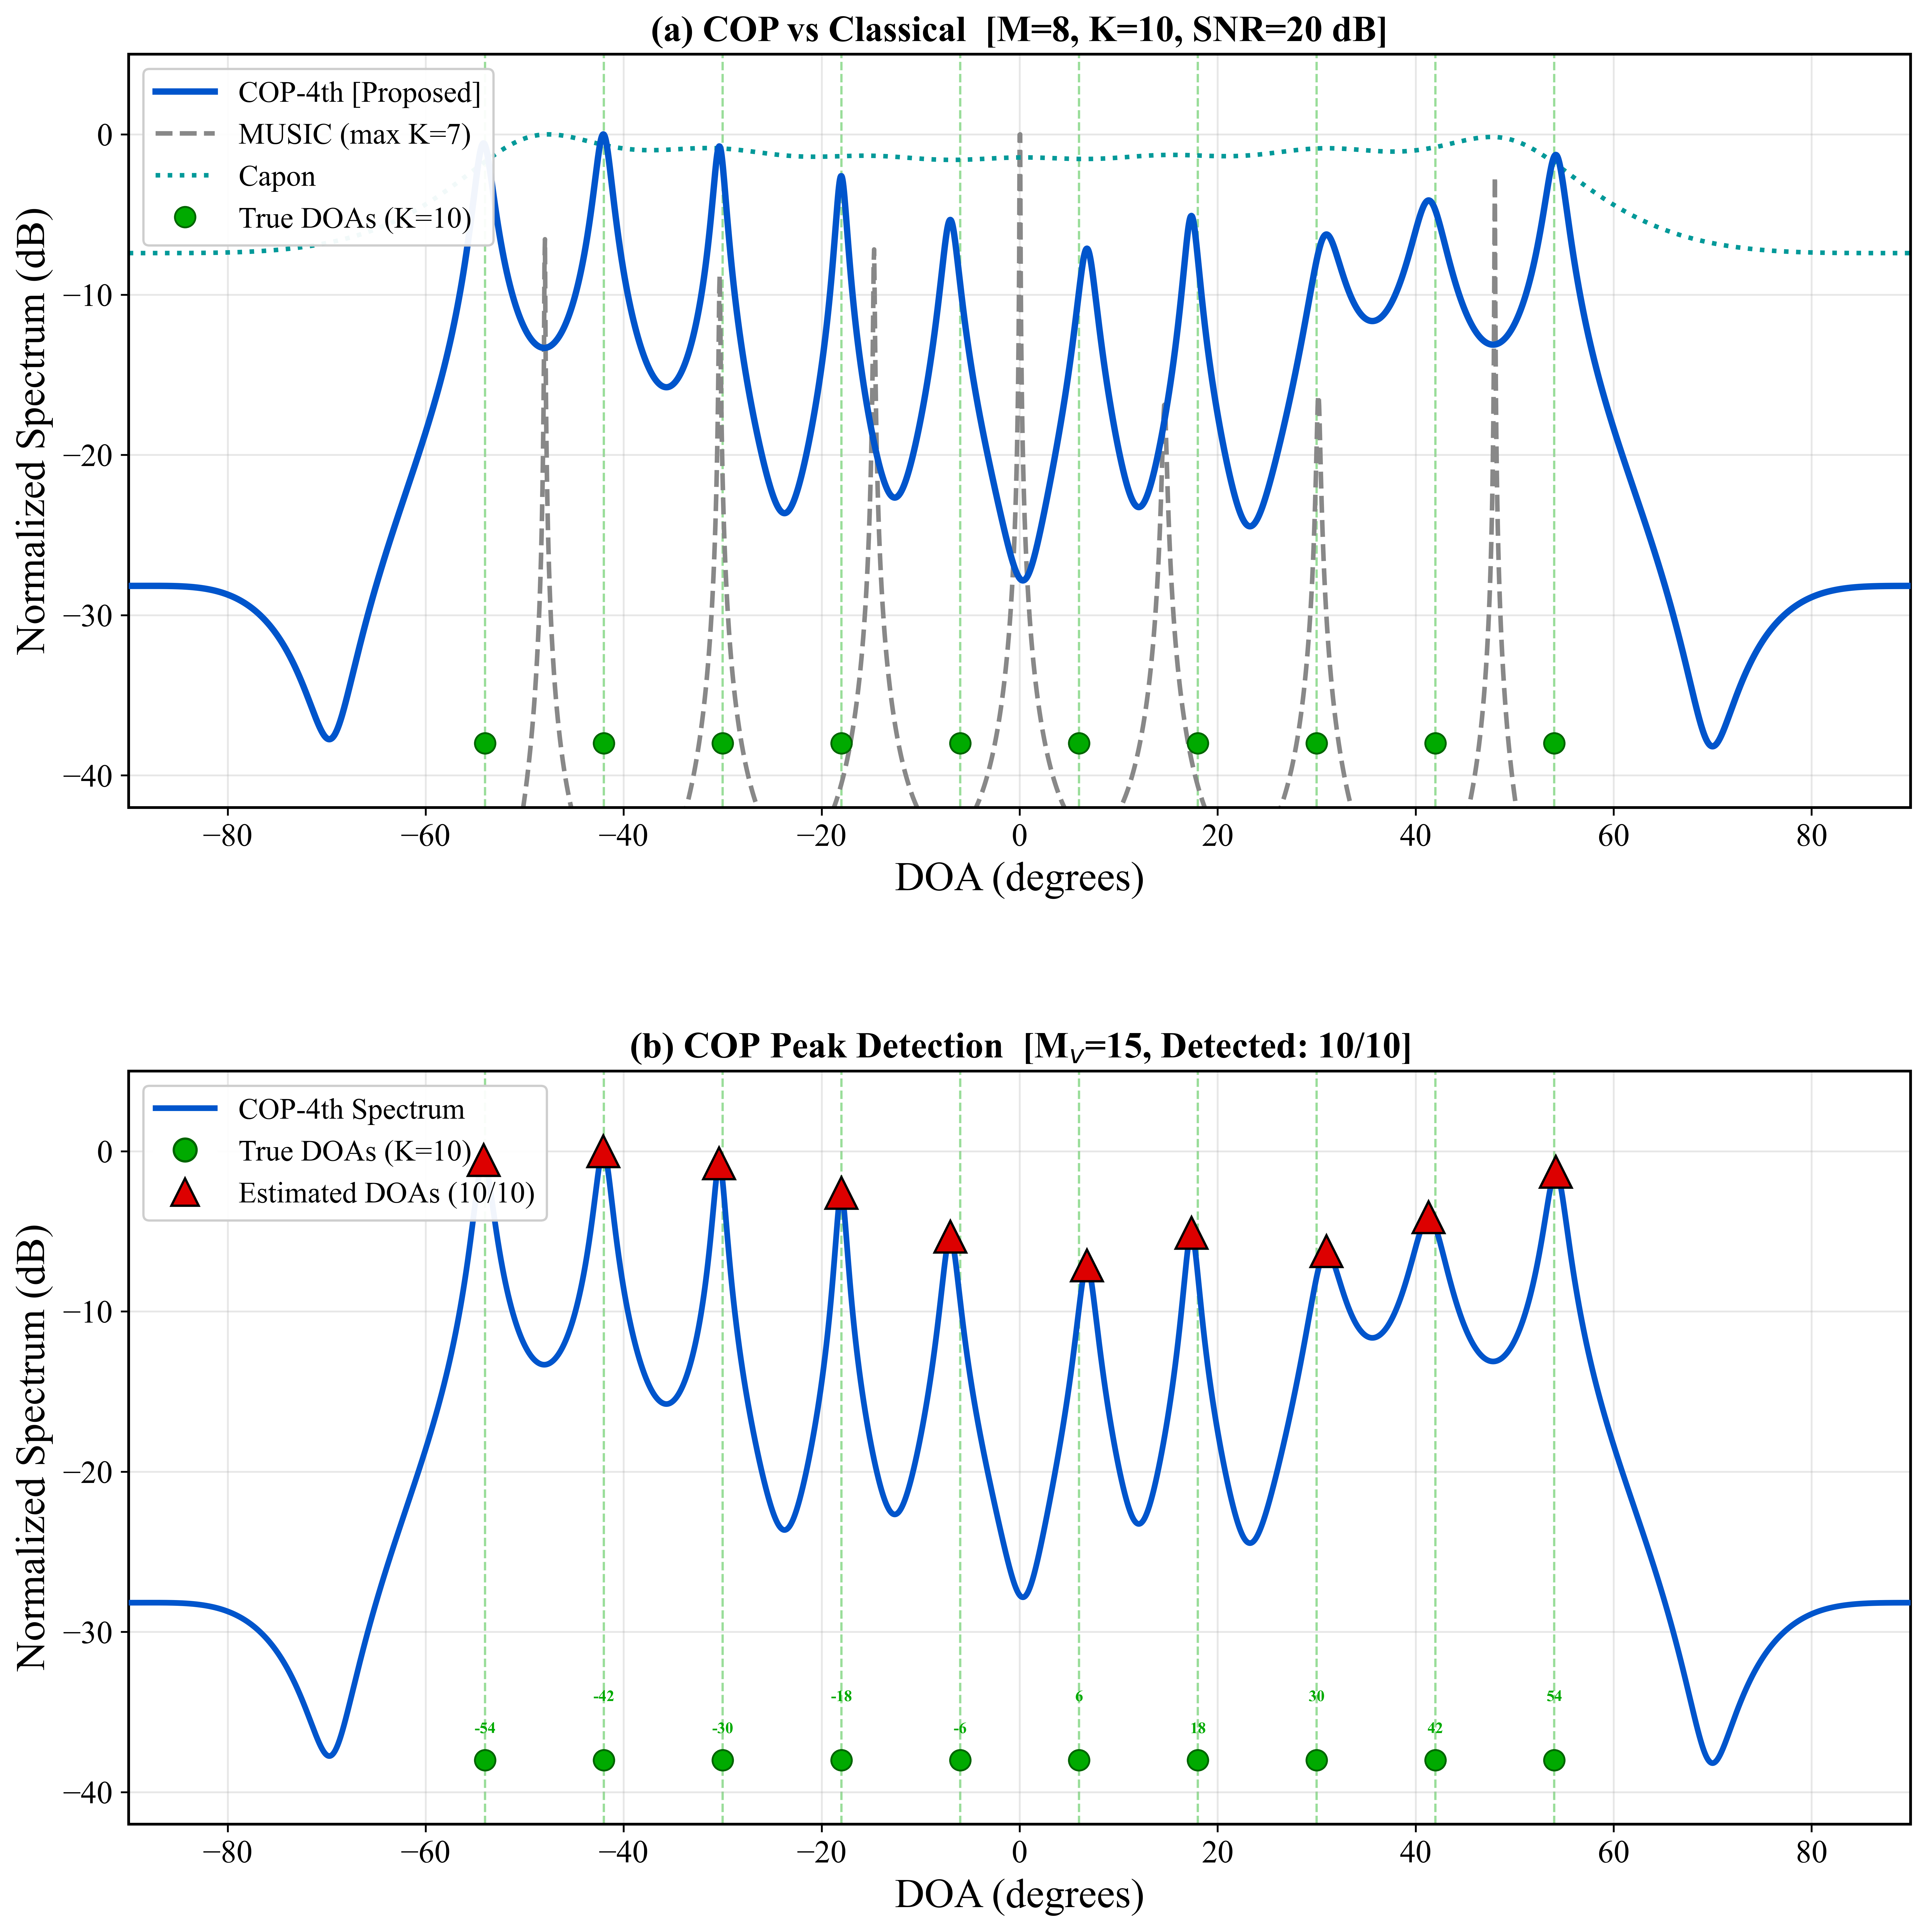
\includegraphics[width=\linewidth]{figures/fig0_spatial_spectrum.png}
\caption{Spatial spectrum for $K=10$ sources, $M=8$ ($K>M{-}1=7$): COP-4th
resolves all sources via the virtual aperture, while MUSIC and Capon fail.
(Top) pseudo-spectra; (bottom) COP peak detection.}
\label{fig:spectrum}
\end{figure}

\begin{table}[t]
\centering
\caption{Underdetermined end-to-end ($K{=}10>M{-}1{=}7$, $500$ trials).}
\label{tab:underdet}
\small
\resizebox{\columnwidth}{!}{%
\begin{tabular}{@{}lcccc@{}}
\toprule
Pipeline & $P_d$ (\%) & locRMSE ($^\circ$) & GOSPA ($^\circ$) & Switches \\
\midrule
COP-RFS   & $\mathbf{60.3\pm0.2}$ & $3.00\pm0.02$ & $16.69\pm0.04$ & $187\pm3$ \\
MUSIC-PHD & $51.9\pm0.1$ & $\mathbf{2.61\pm0.01}$ & $\mathbf{15.39\pm0.01}$ & $\mathbf{66\pm2}$ \\
\bottomrule
\end{tabular}}
\end{table}

Fig.~\ref{fig:pdk} sweeps the front-end detection rate over $K$ (estimator only,
no tracker). The two methods are indistinguishable for $K\le M{-}1=7$, but at
$K=8$ MUSIC collapses (from $100\%$ to $49\%$) and remains near its $(M{-}1)/K$
ceiling, whereas COP degrades only gradually toward the virtual-array limit
$\rho(M{-}1)=14$. The sharp divergence at $K=7$ is the structural signature of
the extended aperture and confirms that the advantage stems from the array
structure rather than from parameter tuning. (The raw front-end rate at $K=10$---about $25\%$
for MUSIC---is lower than the $52\%$ of the end-to-end MUSIC--PHD in
Table~\ref{tab:underdet}: the tracker recovers some detections through temporal
integration and coasting, but cannot create measurements for the structurally
unresolvable sources.)

\begin{figure}[t]
\centering
\includegraphics[width=\linewidth]{figures/fig_pd_vs_k.png}
\caption{Front-end detection rate vs.\ source count $K$ ($M=8$, SNR$=15$~dB,
$T=512$, $60$ trials, $95\%$ CIs). MUSIC collapses for $K>M{-}1=7$ toward its
$(M{-}1)/K$ capacity, while COP-4th sustains detection up to the virtual-array
limit $\rho(M{-}1)=14$.}
\label{fig:pdk}
\end{figure}

\subsection{The Closed Loop is Front-End-Agnostic}
\label{sec:exp_loop}

We next isolate the closed loop via a $2\times2$ (front-end $\times$ loop)
study in the regime where Theorem~2's prior-accuracy condition holds: low SNR
($5$~dB), slowly varying targets ($K=6$). Fig.~\ref{fig:loop2x2} and
Table~\ref{tab:loop2x2} show that the tracker-aided refinement \emph{lowers the
localization error of both front-ends}---COP from $0.71^\circ$ to $0.31^\circ$
($-56\%$) and MUSIC from $0.09^\circ$ to $0.05^\circ$ ($-44\%$). The closed loop
is therefore a front-end-agnostic principle, exactly as predicted by Theorem~2,
rather than a COP-specific mechanism. The larger COP improvement
($-56\%$ vs.\ $-44\%$) is the loop paying down precisely the fourth-order
variance penalty of the higher-order front-end (Section~\ref{sec:signal_model}),
realizing the extended aperture and Gaussian-noise immunity of HOS at a variance
approaching that of second-order MUSIC. This synergy---higher-order statistics
made practical \emph{within} a closed loop---is the central message of the paper. (In this
\emph{determined} regime the lower-variance MUSIC front-end is the more accurate
of the two, consistent with Section~\ref{sec:exp_underdet}.)

\begin{figure}[t]
\centering
\includegraphics[width=0.85\linewidth]{figures/fig_loop_2x2.png}
\caption{Closed-loop refinement improves both the cumulant (COP) and covariance
(MUSIC) front-ends (stationary, SNR$=5$~dB, $K=6$). Bars: matched-pair
localization RMSE; error bars are $95\%$ CIs.}
\label{fig:loop2x2}
\end{figure}

\begin{table}[t]
\centering
\caption{$2\times2$ front-end $\times$ loop (stationary, SNR$=5$~dB, $K=6$).}
\label{tab:loop2x2}
\small
\begin{tabular}{@{}lcc@{}}
\toprule
Front-end & open-loop locRMSE & closed-loop locRMSE \\
\midrule
COP   & $0.71\pm0.02$ & $\mathbf{0.31\pm0.01}$ \\
MUSIC & $0.09\pm0.00$ & $\mathbf{0.05\pm0.00}$ \\
\bottomrule
\end{tabular}
\end{table}

This gain persists across the determined regime. Fig.~\ref{fig:snrdet} sweeps SNR
at $K=6$: the closed loop lowers COP's localization error at \emph{every} SNR (by
about half), while MUSIC's gain is large at low SNR and vanishes as SNR grows---
precisely the $1/(1{+}\kappa)$ behaviour of Theorem~2, since the prior helps most
when the data subspace is noisy ($\kappa$ large). COP benefits more than MUSIC at
all SNR because its fourth-order variance keeps $\kappa$ large; this is the
higher-order-statistics--closed-loop synergy of Section~\ref{sec:signal_model}
made quantitative. Hence the closed loop is useful \emph{even where MUSIC is
applicable}, not only in the underdetermined regime. Importantly, the
\emph{deployed} gated variant (GCL) matches the full closed loop throughout---its
velocity gate engages for these slow targets---so the practical system, not
merely the idealized loop, attains the determined-regime gain.

\begin{figure}[t]
\centering
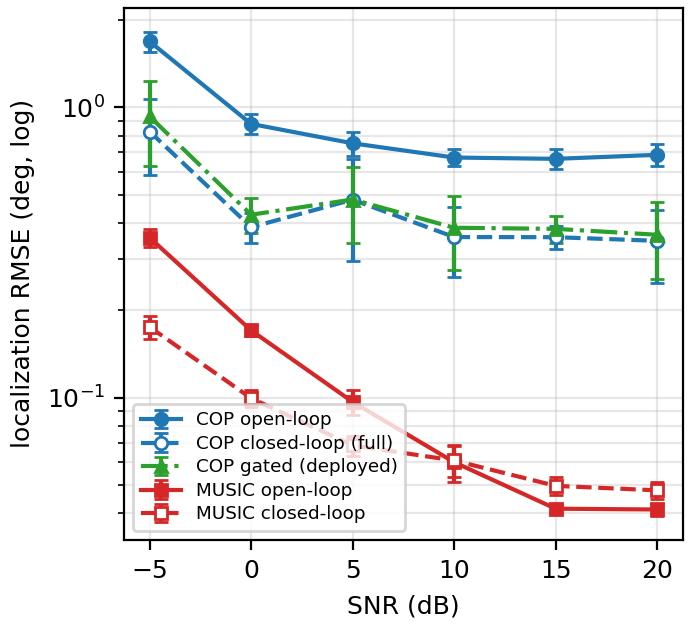
\includegraphics[width=\linewidth]{figures/fig_snr_determined.png}
\caption{Determined regime ($K=6<M{-}1$): localization RMSE vs.\ SNR for COP and
MUSIC (open- and closed-loop) plus the deployed gated COP (GCL), which overlaps
the full closed loop ($30$ trials, $95\%$ CIs). The closed loop helps both
front-ends---most at low SNR---and helps COP at every SNR because its higher-order
variance keeps the prior informative.}
\label{fig:snrdet}
\end{figure}

\subsection{Robustness to Target Motion}
\label{sec:exp_gate}

The temporal accumulation that drives the closed-loop gain is valid only for
slowly varying targets: for fast targets it smears the moving sources and the
accumulating loop \emph{collapses}. In a determined crossing ($K=4$,
$2.5^\circ$/scan) the full closed loop drops $P_d$ from $80.4\%$ to $14.6\%$, and
in the underdetermined scenario from $60.3\%$ to $44.6\%$ (MUSIC's closed loop
degrades identically). The remedy reflects the tracker's motion model into the
prior: we feed back the constant-velocity \emph{prediction}
$\theta+\dot{\theta}\,\Delta t$ instead of the one-scan-lagged current estimate,
and disable accumulation, so the prior matches the current target position even
under motion (Theorem~2's bias $\|\mat{b}\|$ is then governed by the prediction
error, not by the displacement). This motion-compensated refinement is
\emph{safe at arbitrary speed}: on the same $K=4$ crossing it tracks open-loop COP
across SNR$\,\in\{0,5,15\}$~dB ($P_d=77.9$--$79.4\%$ vs.\ open-loop
$78.3$--$80.4\%$, no collapse). A naive velocity-\emph{gated} accumulation cannot
achieve this, because the smear it is meant to suppress also corrupts the velocity
estimate the gate relies on---a circular dependency the prediction-prior variant
sidesteps. The deployed system therefore uses temporal accumulation for slowly
varying targets (the gain of Section~\ref{sec:exp_loop}) and the
motion-compensated refinement otherwise, so the closed loop improves estimation
when the prior is informative and never degrades it.

Beyond doing no harm, the motion-compensated loop yields a genuine \emph{identity}
benefit for moving targets. On the underdetermined moving scenario ($K=10$), at
matched detection ($P_d\approx52\%$) and localization, it reduces label switches
from $214\pm9$ to $181\pm10$ ($-15\%$, non-overlapping $95\%$ CIs): the
prediction-aligned estimates stabilize the tracker's data association through
crossings. The closed loop's value for moving targets is thus in \emph{track
continuity}, not per-scan localization (which the tracker's own filtering already
optimizes)---complementing its detection gain in the underdetermined regime and
its estimation gain in the low-SNR/slow regime.

Table~\ref{tab:cl_efficacy} consolidates these results into a single statement of
the closed loop's efficacy. The temporal feedback delivers a \emph{concrete,
quantified gain in every regime where the prior is informative}: it restores
identifiability where the open-loop bound diverges (Theorem~1), \emph{halves}
COP's low-SNR localization error ($-56\%$), and \emph{cuts moving-target identity
switches by $15\%$}---while the validation gate (Theorem~2) and the
motion-compensated prior guarantee it \emph{never degrades} the open-loop baseline
where the prior is not. This asymmetry---real gains when the prior helps, provable
no-harm when it does not---is the practical case for closing the loop.

\begin{table}[t]
\centering
\caption{Closed-loop efficacy: quantified gain over the open-loop cascade. Each
entry is substantiated, with $95\%$ CIs, in the cited theorem/section.}
\label{tab:cl_efficacy}
\small
\resizebox{\columnwidth}{!}{%
\begin{tabular}{@{}llcc@{}}
\toprule
Benefit (where) & Metric & Open-loop & Closed-loop \\
\midrule
Identifiability, $K\!\to\!M_v{-}1$ (Thm~1) & PCRB & diverges & \textbf{finite} \\
Localization, COP @ $5$~dB (\S\ref{sec:exp_loop}) & locRMSE & $0.71^\circ$ & $\mathbf{0.31^\circ}$ \,($-56\%$) \\
Localization, MUSIC @ $5$~dB (\S\ref{sec:exp_loop}) & locRMSE & $0.09^\circ$ & $\mathbf{0.05^\circ}$ \,($-44\%$) \\
Track continuity, moving $K{=}10$ (\S\ref{sec:exp_gate}) & switches & $214$ & $\mathbf{181}$ \,($-15\%$) \\
Fast motion, safety (\S\ref{sec:exp_gate}) & $P_d$ & baseline & \textbf{no loss} \\
\bottomrule
\end{tabular}}
\end{table}

\subsection{Validation of the Theory}
\label{sec:exp_theory}

\textbf{Closed-loop posterior CRB (Theorem~1).}
Fig.~\ref{fig:pcrb} plots the worst-case angle bound versus source count. The
open-loop (data-only) bound diverges as $K$ approaches the virtual-array limit
$M_v-1$, whereas the closed-loop PCRB~\eqref{eq:pcrb} remains bounded by the
prior information $1/\lambda_{\min}(\mat{J}_{k|k-1})$, confirming that the
temporal prior restores identifiability. In the well-determined regime the two
bounds coincide, matching the regime delineation above.

\begin{figure}[t]
\centering
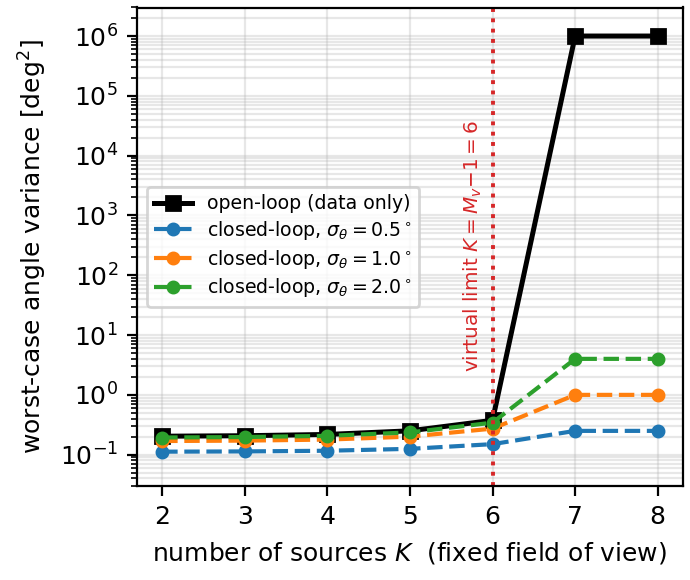
\includegraphics[width=0.92\linewidth]{figures/fig_pcrb_validation.png}
\caption{Validation of Theorem~1: open-loop bound diverges at the virtual-array
limit while the closed-loop PCRB stays finite; near-parity in the
well-determined regime.}
\label{fig:pcrb}
\end{figure}

\textbf{Minimum-variance refinement (Theorem~2).}
Fig.~\ref{fig:tcopmse} validates~\eqref{eq:tcopB}--\eqref{eq:tcop_bias}: the
fused subspace MSE matches the predicted improvement factor $1/(1+\kappa)$ for an
unbiased prior, and the empirical break-even point of the biased case lands at
$\|\mat{b}\|^2=D(\sigma_e^2+\sigma_p^2)$, with the validation gate keeping the
fused MSE at or below the data-only MSE.

\begin{figure}[t]
\centering
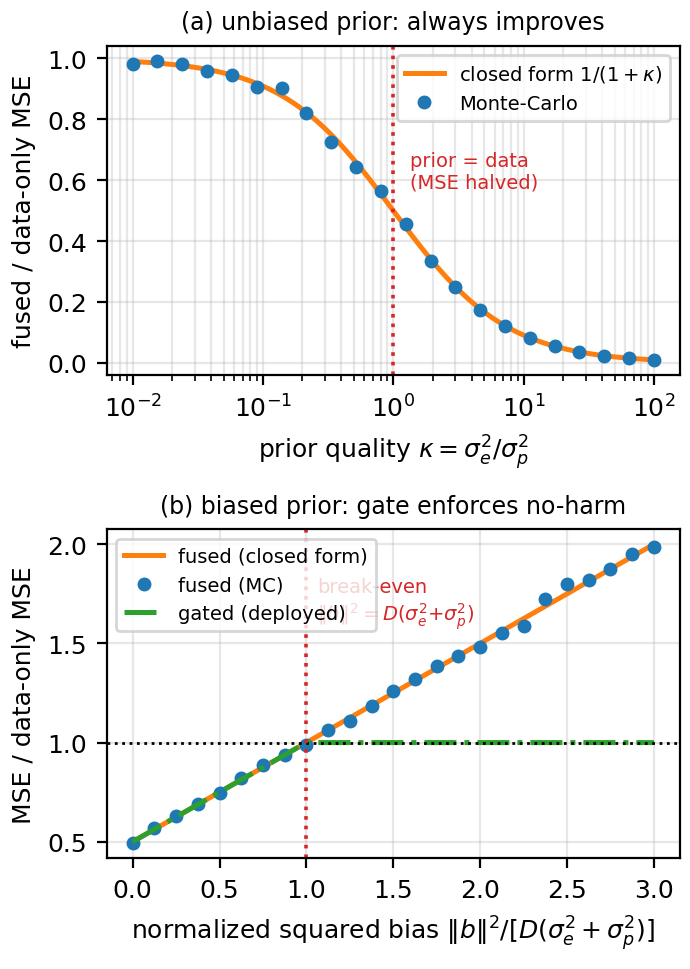
\includegraphics[width=\linewidth]{figures/fig_tcop_mse_validation.png}
\caption{Validation of Theorem~2: (left) unbiased-prior MSE follows $1/(1+\kappa)$;
(right) biased-prior break-even at $\|\mat{b}\|^2=D(\sigma_e^2+\sigma_p^2)$ and
the gated estimator never exceeds the data-only MSE.}
\label{fig:tcopmse}
\end{figure}

\subsection{Identity Preservation at Crossings}
\label{sec:exp_cross}

Finally we evaluate the tracking back-end on the COP front-end ($K=4$ crossing
targets, $30$ scans, $40$ trials), comparing our track-oriented TO-PHD against the
standard GM-PHD~\cite{vo2006gmphd}, the labeled multi-Bernoulli (LMB)
filter~\cite{vo2014lmb}, and the full $\delta$-GLMB filter~\cite{vo2013glmb}
implemented with the Gibbs-sampling truncation of~\cite{vo2017efficient}---the
state-of-the-art labeled-RFS trackers requested in review.
Table~\ref{tab:ablation} shows that all three \emph{labeled} filters reduce
identity switches by an order of magnitude over the unlabeled GM-PHD ($17$--$37$
vs.\ $385$), whose first-moment recursion coalesces tracks at crossings, while all
four attain comparable detection ($80$--$82\%$, Proposition~1). Among the labeled
trackers, the full $\delta$-GLMB---which propagates the joint distribution over
label-to-measurement association histories that LMB approximates by its
marginals---attains the \emph{cleanest identity} (fewest switches, $17\pm2$) and
the \emph{sharpest matched localization} (locRMSE $0.91^\circ$), consistent with
its status as the exact labeled filter; LMB attains the best aggregate GOSPA, its
marginally higher detection offsetting $\delta$-GLMB's localization edge. The
small $\delta$-GLMB--LMB gap confirms LMB as a faithful, cheaper approximation,
and our physics-based TO-PHD is a competitive lightweight alternative (no
association-hypothesis sampling). Crucially, the COP-RFS framework is
\emph{agnostic to the back-end}: the closed-loop higher-order front-end of
Sections~\ref{sec:exp_underdet}--\ref{sec:exp_loop} can drive any RFS tracker, and
moving from TO-PHD to LMB or $\delta$-GLMB trades computation for identity
accuracy. We do not claim TO-PHD is the optimal tracker---the labeled-RFS filters
are more accurate---but that the framework's contributions are orthogonal to, and
compatible with, the choice of back-end. (This determined crossing stresses
identity; the COP front-end's advantage lies in the underdetermined regime of
Section~\ref{sec:exp_underdet}.) A summary of the operating regimes is given in
Table~\ref{tab:regime}.

\begin{table}[t]
\centering
\caption{Tracking back-end ablation on the COP front-end ($K{=}4$ crossing, $40$ trials, $95\%$ CIs). All three labeled filters cut switches $\sim$20$\times$ vs.\ GM-PHD; $\delta$-GLMB gives the cleanest identity and sharpest localization, LMB the best aggregate GOSPA.}
\label{tab:ablation}
\small
\resizebox{\columnwidth}{!}{%
\begin{tabular}{@{}lcccc@{}}
\toprule
Back-end & $P_d$ (\%) & locRMSE ($^\circ$) & GOSPA ($^\circ$) & Switches \\
\midrule
Standard GM-PHD~\cite{vo2006gmphd} & $82.3\pm0.7$ & $1.35\pm0.08$ & $6.12\pm0.14$ & $385\pm8$ \\
TO-PHD (ours)                      & $80.4\pm0.6$ & $1.03\pm0.09$ & $5.42\pm0.21$ & $37\pm6$ \\
LMB~\cite{vo2014lmb}               & $81.6\pm0.8$ & $0.96\pm0.07$ & $\mathbf{5.22\pm0.17}$ & $24\pm3$ \\
$\delta$-GLMB~\cite{vo2013glmb,vo2017efficient} & $80.6\pm0.8$ & $\mathbf{0.91\pm0.07}$ & $5.35\pm0.17$ & $\mathbf{17\pm2}$ \\
\bottomrule
\end{tabular}}
\end{table}

\begin{table}[t]
\centering
\caption{Operating-regime summary: where each ingredient helps.}
\label{tab:regime}
\small
\resizebox{\columnwidth}{!}{%
\begin{tabular}{@{}lll@{}}
\toprule
Regime & Best front-end & Closed loop \\
\midrule
Determined ($K\le M{-}1$) & MUSIC (2nd-order) & helps (if prior accurate) \\
Underdetermined ($K>M{-}1$) & COP (higher-order) & helps; gate if fast \\
Low SNR, slow/stationary & either & strongly helps \\
Fast motion & open-loop & gated off (no harm) \\
\bottomrule
\end{tabular}}
\end{table}

\section{Conclusion}
\label{sec:conclusion}

This paper presented COP-RFS, a closed-loop framework that couples higher-order-cumulant DOA estimation with RFS-based multi-target tracking and, unlike prior open-loop cascades, analyzes the coupling itself. The central message is that the tracker's temporal prediction is information the open-loop pipeline discards, and that feeding it back is provably beneficial \emph{in a characterized regime} rather than uniformly. Concretely (Table~\ref{tab:cl_efficacy}), the closed loop restores identifiability where the data-only bound diverges (Theorem~1), halves COP's low-SNR localization error ($-56\%$), and cuts moving-target identity switches by $15\%$, while a validation gate and a motion-compensated prior guarantee it never degrades the open-loop baseline.

The key contributions and findings are:
\begin{enumerate}
\item \textbf{Closed-loop posterior CRB}: Theorem~1 gives the first CRB for the complete coupled estimator--tracker and shows that the temporal prior strictly tightens the bound, restoring identifiability exactly in the underdetermined regime where the data-only bound diverges.
\item \textbf{Provably minimum-variance refinement}: Theorem~2 recasts T-COP subspace refinement as a basis-invariant Grassmann inverse-variance fusion and proves it is minimum-variance under an explicit prior-accuracy condition; a validation gate enforces this condition, so the closed loop improves estimation when the prior is accurate and never degrades it otherwise.
\item \textbf{Underdetermined capability, honestly bounded}: With Monte-Carlo evaluation (up to $500$ trials) and $95\%$ confidence intervals, and against MUSIC, closed-loop-MUSIC, labeled multi-Bernoulli (LMB), and full $\delta$-GLMB baselines, COP-RFS detects significantly more targets than a MUSIC--PHD cascade when $K>M{-}1$, while the track-oriented PHD back-end preserves identity through crossings; the closed loop is demonstrated to be both front-end- and back-end-agnostic. We explicitly delineate the operating regime---low SNR and slow target motion for the closed-loop estimation gain, $K>M{-}1$ for the detection gain---rather than claiming uniform superiority; SD-COP extends operation toward the super-underdetermined regime.
\end{enumerate}

The proposed framework is particularly relevant to defense, speech enhancement, and communications applications where multiple targets must be simultaneously detected and tracked using compact sensor arrays.

Future directions include: (i)~extension to 2-D (azimuth--elevation) DOA with uniform rectangular arrays for full spatial tracking; (ii)~environment-adaptive motion models accounting for altitude-dependent atmospheric density and drag coefficients in defense scenarios; and (iii)~real-time embedded implementation with operational radar hardware.

% Acknowledgment
\section*{Acknowledgment}
This work utilized Claude (Anthropic) as an AI assistant for code development, experimental automation, and manuscript preparation including \LaTeX{} formatting and text editing. All scientific content, theoretical derivations, algorithmic design, and experimental interpretation were solely conducted by the authors.

% References
\bibliographystyle{IEEEtran}
\bibliography{references_R1}

\end{document}
